
\section{WENO methods for the Euler equations}
\label{sec:weno-euler}

When dealing with nonlinear systems the flux split method introduced in
section~\ref{sec:weno-burgers-fvs} generalizes directly. The simplest, and most
diffusive flux splitting uses the maximum characteristic speed $\alpha$. For a
system, such as the Euler equations, the simplest method is to compute $\alpha$
by maximizing over all characteristics. The directional fluxes $\Fb^{(\pm)}(u)$
can then be reconstructed using a high order WENO scheme component by component.

However, this approach can lead to significant oscillations, even in moderate
tests. Rather than doing the reconstruction of the components of the directional
fluxes, a safer approach is to work with characteristic variables. The
discussion in chapter~\ref{ch:compressible-theory} suggests that, by computing
the left and right eigenvectors of the appropriate Jacobian matrix
$\Ab = \partial \Fb/\partial \Uc$, we can project the directional fluxes into
the directional \emph{characteristic} fluxes (using the left eigenvectors),
reconstruct these characteristic fluxes using a high order method, and then
compute the reconstructed directional fluxes required (using the right
eigenvectors). As the characteristic fluxes should contain information about
only a single wave at a time, this \emph{should} give similar results to the
scalar case and reduce problems from close waves from different families.

The Jacobian matrix needs to be computed separately for each point at which the
flux needs computing. The best choice of state from which the Jacobian is
computed is not clear: often the arithmetic average of neighbouring states is
used, but more complex choices can give better results.

A direct comparison of component-wise and characteristic-wise flux-vector split
WENO methods, applied to the Sod test, is given in
figure~\ref{fig:weno-euler-r3} for $r=3$ and in figure~\ref{fig:weno-euler-r5}
for $r=5$. The comparison to the PPM method in figure~\ref{fig:Euler:sod:ppm} is
particularly instructive. The PPM method is specifically designed for
hydrodynamic problems, and is much better at cleanly capturing the
discontinuities, especially the contact. The WENO approach will have a higher
order of accuracy, which will be clearest on tests with more smooth variation.
The oscillations introduced by the WENO methods are more pronounced as the
order is increased, but are reduced by the use of characteristic-wise
reconstruction. This is most clearly seen in the results for the internal energy
in the $r=5$ case shown in figure~\ref{fig:weno-euler-r5}.

\begin{figure}[t]
\centering
% figure generated by hydro_examples/compressible/weno-euler.py
\includegraphics[width=0.8\linewidth]{weno-euler-r3}
\caption[WENO $r=3$ for the Sod test]
{\label{fig:weno-euler-r3} The Sod test solved with WENO methods, $r=3$, using characteristic-wise and component-wise reconstruction, using 64 zones and a cfl of $0.5$. To compare with Godunov's method see figure~\ref{fig:Euler:sod:god} and with PPM see figure~\ref{fig:Euler:sod:ppm}. The WENO method does not capture discontinuities, especially the contact, as well as the PPM method which is specifically designed for the Euler equations. The small oscillations visible in the component-wise reconstruction are damped by using the more complex and expensive characteristic-wise approach. \\
\hydroexdoit{\href{https://github.com/zingale/hydro_examples/blob/master/compressible/weno_euler.py}{weno\_euler.py}}}
\end{figure}
%

\begin{figure}[t]
\centering
% figure generated by hydro_examples/compressible/weno-euler.py
\includegraphics[width=0.8\linewidth]{weno-euler-r5}
\caption[WENO $r=5$ for the Sod test]
{\label{fig:weno-euler-r5} The Sod test solved with WENO methods, $r=5$, using characteristic-wise and component-wise reconstruction, using 64 zones and a cfl of $0.5$. Compare with figure~\ref{fig:weno-euler-r3} to see the effect of the higher order of WENO scheme. The oscillations in the component-wise approach are much more pronounced as the order of the reconstruction is increased, and the characteristic-wise approach continues to help with this. \\
\hydroexdoit{\href{https://github.com/zingale/hydro_examples/blob/master/compressible/weno_euler.py}{weno\_euler.py}}}
\end{figure}
%

Another illustration of the advantages of a numerical method, such as PPM, that
is specifically designed for the Euler equations, is shown in the double
rarefaction test in figure~\ref{fig:weno-euler-rarefaction-r3}. The
advantages of the higher order methods are shown by how well the WENO schemes
capture the edges of the rarefaction waves, even with so few points and the
diffusive Lax-Friedrichs flux splitting. However, the artificial heating effect
seen at the trivial contact at the center of the domain is about as bad as that
from piecewise constant reconstruction, and nowhere near as good as PPM. Whilst
increasing the reconstruction order has a small impact, a less diffusive flux
splitting would be needed to approach PPM's performance.

\begin{figure}[t]
\centering
% figure generated by hydro_examples/compressible/weno-euler.py
\includegraphics[width=0.8\linewidth]{weno-euler-rarefaction-r3}
\caption[WENO $r=3$ for the double rarefaction test]
{\label{fig:weno-euler-rarefaction-r3} The double rarefaction test solved with WENO methods, $r=3$, using characteristic-wise and component-wise reconstruction, using 64 zones and a cfl of $0.5$. To compare with Godunov's method see figure~\ref{fig:Euler:doublerare:god} and with PPM see figure~\ref{fig:Euler:doublerare:ppm}. The WENO method captures the edges of the rarefactions almost as well as the PPM method, but is as almost as poor as Godunov's method at the trivial contact at the center. A less diffusive flux-splitting may help here. Increasing the reconstruction order has little effect.\\
\hydroexdoit{\href{https://github.com/zingale/hydro_examples/blob/master/compressible/weno_euler.py}{weno\_euler.py}}}
\end{figure}
%

\subsection{Extensions}

The main advantage of the WENO method is that it retains its high order when
extending to multiple dimensions using dimensional splitting. From the
finite-difference form there are no transverse Riemann problems to solve. From
using the Method of Lines there is no issue about ordering the dimensional
sweeps: the updates in each direction are computed separately but applied
together in the time integrator. This formally retains the high-order accuracy
but can lose significant absolute accuracy -- compare the advection of a
top-hat function with lower order methods using transverse Riemann problem
solutions.

The global Lax-Friedrichs flux splitting above can be excessively diffusive. A
local Lax-Friedrichs flux splitting, where $\alpha$ is computed at each point
by maximising over the characteristic speed within the stencil at that point, is
less diffusive but slightly more expensive. Roe-style flux splittings are
possible but not always stable.


\section{Discontinuous Galerkin methods for the Euler equations}
\label{sec:dg_euler}

The Discontinuous Galerkin methods introducted in section~\ref{sec:dg} extend to
nonlinear systems directly. For a nonlinear scalar conservation law,
%
\begin{equation}
  q_t + f(q)_x = 0,
\end{equation}
%
the Discontinuous Galerkin method becomes
%
\begin{equation}
  \label{eq:dg_nodal_scalar_nonlinear}
  M \ddt{\bm{\hat{q}}} + S^T f (\bm{\hat{q}}) = -\left[ \bm{\psi F} \right]_{x_{j-1/2}}^{x_{j+1/2}}.
\end{equation}
%
This should be compared with equation~\eqref{eq:dg_nodal_final}
%
\begin{equation}
  \tag{\ref{eq:dg_nodal_final}}
  M \ddt{\bm{\hat{a}}} + S^T u \bm{\hat{a}} = -\left[ \bm{\psi F} \right]_{x_{j-1/2}}^{x_{j+1/2}}
\end{equation}
%
for the advection equation with advection speed $u$. The crucial change is that
the stiffness matrix $S$ is now multiplying the nonlinear flux term, and the
boundary flux on the right hand side now needs a nonlinear Riemann solver or an
appropriate approximation. The Lax-Friedrichs flux is often used here. Extending
to a system of nonlinear conservation laws means applying the above scheme
component-by-component, either directly to the conserved variables, or by
transforming to the characteristic variables.

\begin{figure}[t]
\centering
% figure generated by hydro_examples/compressible/dg_euler.py
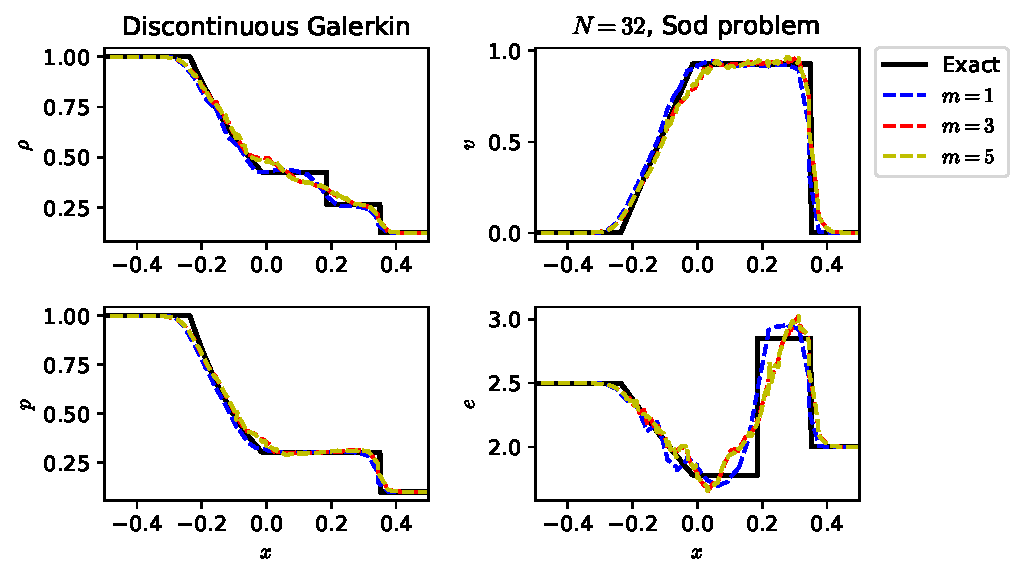
\includegraphics[width=0.8\linewidth]{dg_sod_32}
\caption[Discontinuous Galerkin methods applied to the Sod problem, low resolution]
{\label{fig:dg-euler-sod32} Various Discontinuous Galerkin methods, using moment
limiting, applied to the Sod problem with $N=32$. We see that the method
struggles near discontinuities, and that increasing $m$ alone does not improve
the results.\\
\hydroexdoit{\href{https://github.com/zingale/hydro_examples/blob/master/compressible/dg_euler.py}{dg\_euler.py}}}
\end{figure}
%

\begin{figure}[t]
\centering
% figure generated by hydro_examples/compressible/dg_euler.py
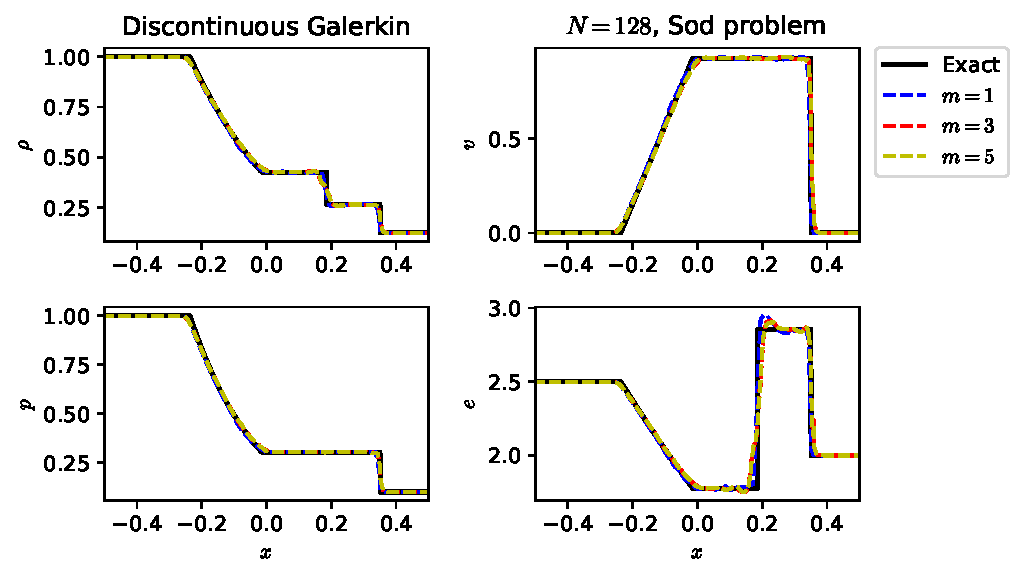
\includegraphics[width=0.8\linewidth]{dg_sod_128}
\caption[Discontinuous Galerkin methods applied to the Sod problem, high resolution]
{\label{fig:dg-euler-sod128} Various Discontinuous Galerkin methods, using moment
limiting, applied to the Sod problem with $N=128$. We see that the method
now has enough resolution to produce good results, but that increasing $m$ alone
still does not improve the results.\\
\hydroexdoit{\href{https://github.com/zingale/hydro_examples/blob/master/compressible/dg_euler.py}{dg\_euler.py}}}
\end{figure}
%

The strength of the Discontinuous Galerkin method is its high order accuracy and
minimal coupling to neighbouring cells. Its weakness is its behaviour near
discontinuities. As many tests of the Euler equations seen above focus on
results involving shocks, we will not see the DG methods at their best. For
example, in Figures~\ref{fig:dg-euler-sod32} and \ref{fig:dg-euler-sod128} the
Sod problem is solved. The DG method and limiting is applied directly to the
conserved variables. At low resolution the method struggles. There are so few
cells covering the shock and contact that it has difficulty clearly resolving
the jumps, although the oscillations are not large enough to be problematic. As
the resolution is increased the results are much improved, but in both cases it
is the increased resolution through the number of grid cells $N$ rather than the
number of modes $m$ that is important. The is in complete contrast with the
smooth solutions seen for the advection equation, where the larger gains were
seen by increasing $m$.

\begin{figure}[t]
\centering
% figure generated by hydro_examples/compressible/dg_euler.py
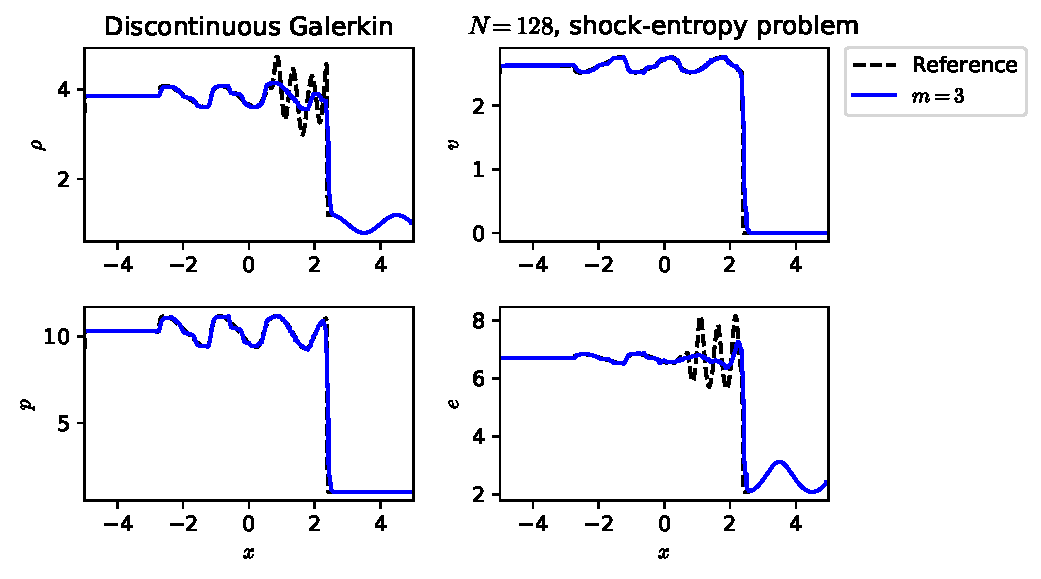
\includegraphics[width=0.8\linewidth]{dg_shock_entropy_m3_N128}
\caption[Discontinuous Galerkin methods applied to the shock-entropy problem, low resolution]
{\label{fig:dg-euler-shockentropy-m3-N128} The shock-entropy interaction problem,
solve using Discontinuous Galerkin methods with moment limiting, with $m=3$ and
$N=128$. We see that the method is excellent at resolving the smooth features to
the right, which have not interacted with the shock. The finer features just
after the shock are not well captured. Modifying $m$ has little effect here. The
reference solution uses a WENO method with $r=4$ and $N=1024$.\\
\hydroexdoit{\href{https://github.com/zingale/hydro_examples/blob/master/compressible/dg_euler.py}{dg\_euler.py}}}
\end{figure}
%

\begin{figure}[t]
\centering
% figure generated by hydro_examples/compressible/dg_euler.py
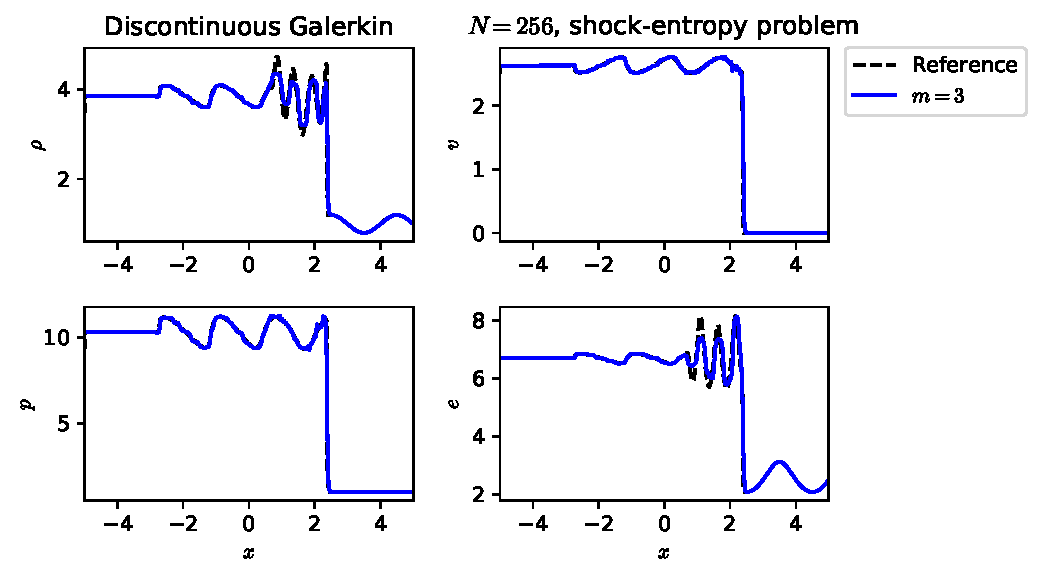
\includegraphics[width=0.8\linewidth]{dg_shock_entropy_m3_N256}
\caption[Discontinuous Galerkin methods applied to the shock-entropy problem, high resolution]
{\label{fig:dg-euler-shockentropy-m3-N256} The shock-entropy interaction problem,
solve using Discontinuous Galerkin methods with moment limiting, with $m=3$ and
$N=256$. The results are similar to Figure~\ref{fig:dg-euler-shockentropy-m3-N128}
but there is now sufficient resolution to capture the finer features after the
shock.\\
\hydroexdoit{\href{https://github.com/zingale/hydro_examples/blob/master/compressible/dg_euler.py}{dg\_euler.py}}}
\end{figure}
%

A test that better captures the advantages as well as the disadvantages of these
methods is the shock-entropy interaction test. A right-going shock interacts
with an entropy wave, with the final results showing both smooth features (that
should be captured well by high order schemes) and shocks (which are more
problematic). Results are shown in Figures~\ref{fig:dg-euler-shockentropy-m3-N128}
and \ref{fig:dg-euler-shockentropy-m3-N256}. The smooth features are mostly
extremely well captured even at these low resolutions, \emph{except} immediately
after the shock. Here again varying $m$ has limited impact, and the crucial
thing is to increase $N$ until the features are resolvable.
